\documentclass{standalone}
\usepackage{tikz}
\usetikzlibrary{patterns, positioning}

\begin{document}
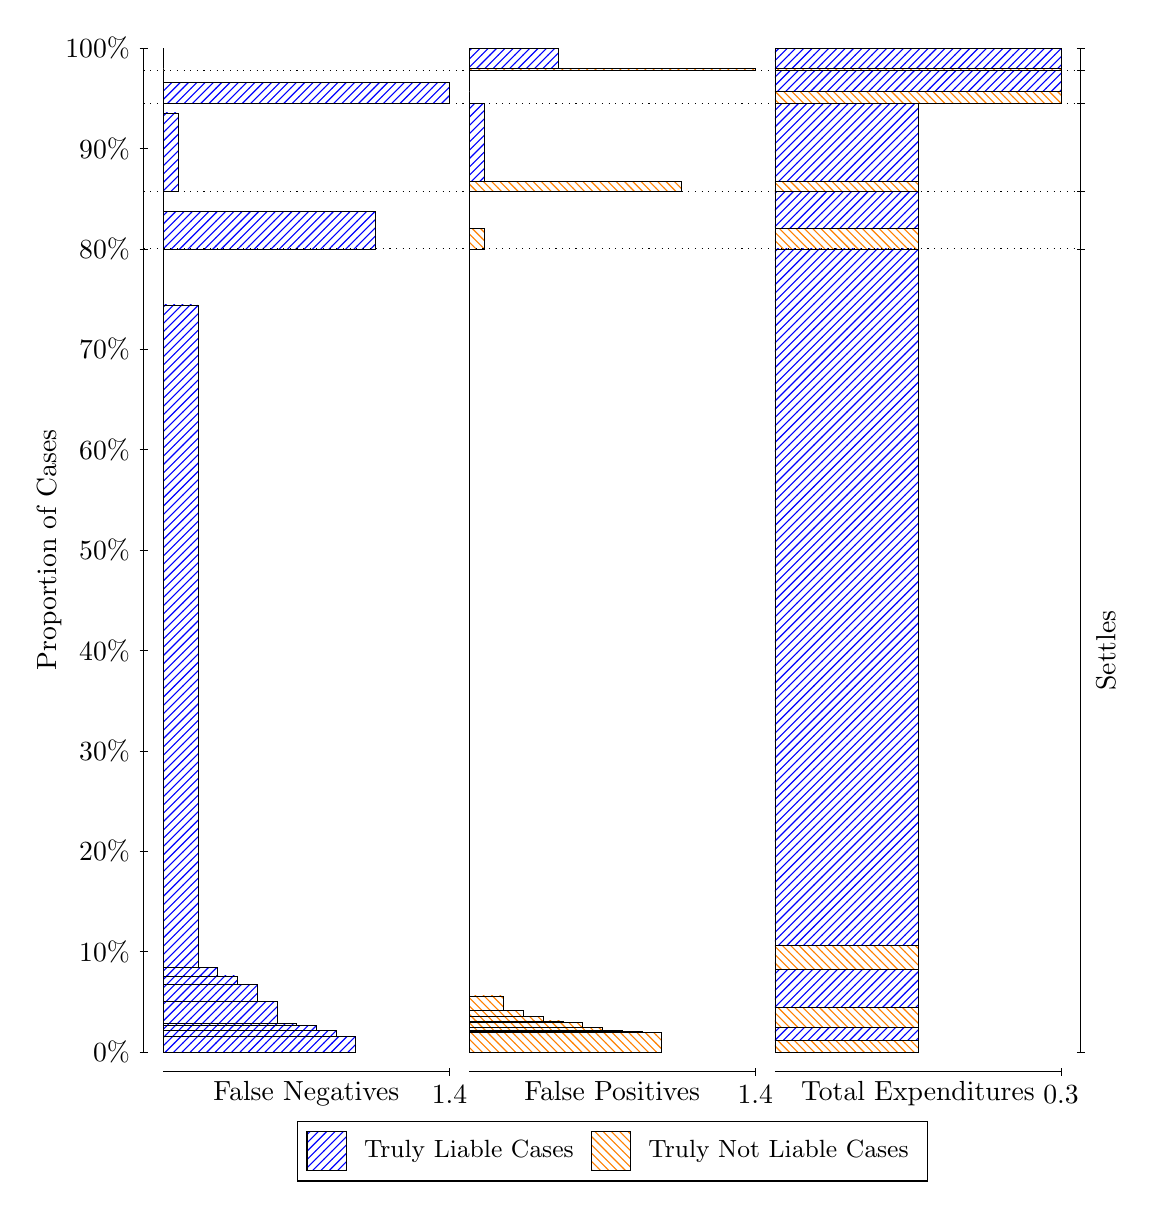
\begin{tikzpicture}
\draw[black, very thin] (1.5,1.75) -- (1.5,14.5);
\node[rotate=90, anchor=center] at (0.3, 8.125) {Proportion of Cases};
\draw[black, very thin] (1.45,1.75) -- (1.55,1.75);
\node[anchor=east] at (1.45, 1.75) {0\%};
\draw[black, very thin] (1.45,3.025) -- (1.55,3.025);
\node[anchor=east] at (1.45, 3.025) {10\%};
\draw[black, very thin] (1.45,4.3) -- (1.55,4.3);
\node[anchor=east] at (1.45, 4.3) {20\%};
\draw[black, very thin] (1.45,5.575) -- (1.55,5.575);
\node[anchor=east] at (1.45, 5.575) {30\%};
\draw[black, very thin] (1.45,6.85) -- (1.55,6.85);
\node[anchor=east] at (1.45, 6.85) {40\%};
\draw[black, very thin] (1.45,8.125) -- (1.55,8.125);
\node[anchor=east] at (1.45, 8.125) {50\%};
\draw[black, very thin] (1.45,9.4) -- (1.55,9.4);
\node[anchor=east] at (1.45, 9.4) {60\%};
\draw[black, very thin] (1.45,10.675) -- (1.55,10.675);
\node[anchor=east] at (1.45, 10.675) {70\%};
\draw[black, very thin] (1.45,11.95) -- (1.55,11.95);
\node[anchor=east] at (1.45, 11.95) {80\%};
\draw[black, very thin] (1.45,13.225) -- (1.55,13.225);
\node[anchor=east] at (1.45, 13.225) {90\%};
\draw[black, very thin] (1.45,14.5) -- (1.55,14.5);
\node[anchor=east] at (1.45, 14.5) {100\%};

\draw[black, very thin] (13.4,1.75) -- (13.4,14.5);
\draw[black, very thin] (13.35,1.75) -- (13.45,1.75);
\node[anchor=west] at (13.35, 1.75) {};
\draw[black, very thin] (13.35,11.949) -- (13.45,11.949);
\node[anchor=west] at (13.35, 11.949) {};
\draw[black, very thin] (13.35,12.681) -- (13.45,12.681);
\node[anchor=west] at (13.35, 12.681) {};
\draw[black, very thin] (13.35,13.798) -- (13.45,13.798);
\node[anchor=west] at (13.35, 13.798) {};
\draw[black, very thin] (13.35,14.213) -- (13.45,14.213);
\node[anchor=west] at (13.35, 14.213) {};
\draw[black, very thin] (13.35,14.5) -- (13.45,14.5);
\node[anchor=west] at (13.35, 14.5) {};

\draw[black, very thin, pattern color=blue, pattern=north east lines] (1.75,1.75) rectangle (4.1931,1.9497);
\draw[black, very thin, pattern color=blue, pattern=north east lines] (1.75,1.9497) rectangle (3.9425,2.0255);
\draw[black, very thin, pattern color=blue, pattern=north east lines] (1.75,2.0255) rectangle (3.692,2.0882);
\draw[black, very thin, pattern color=blue, pattern=north east lines] (1.75,2.0882) rectangle (3.4414,2.1149);
\draw[black, very thin, pattern color=blue, pattern=north east lines] (1.75,2.1149) rectangle (3.1908,2.3937);
\draw[black, very thin, pattern color=blue, pattern=north east lines] (1.75,2.3937) rectangle (2.9402,2.6066);
\draw[black, very thin, pattern color=blue, pattern=north east lines] (1.75,2.6066) rectangle (2.6897,2.7172);
\draw[black, very thin, pattern color=blue, pattern=north east lines] (1.75,2.7172) rectangle (2.4391,2.8232);
\draw[black, very thin, pattern color=blue, pattern=north east lines] (1.75,2.8232) rectangle (2.1885,11.237);
\draw[black, very thin, pattern color=orange, pattern=north west lines] (1.75,11.237) rectangle (1.75,11.949);
\draw[black, very thin, pattern color=blue, pattern=north east lines] (1.75,11.949) rectangle (4.4437,12.422);
\draw[black, very thin, pattern color=orange, pattern=north west lines] (1.75,12.422) rectangle (1.75,12.681);
\draw[black, very thin, pattern color=blue, pattern=north east lines] (1.75,12.681) rectangle (1.9379,13.676);
\draw[black, very thin, pattern color=orange, pattern=north west lines] (1.75,13.676) rectangle (1.75,13.798);
\draw[black, very thin, pattern color=blue, pattern=north east lines] (1.75,13.798) rectangle (5.3833,14.06);
\draw[black, very thin, pattern color=orange, pattern=north west lines] (1.75,14.06) rectangle (1.75,14.213);
\draw[black, very thin, pattern color=orange, pattern=north west lines] (1.75,14.213) rectangle (1.75,14.241);
\draw[black, very thin, pattern color=blue, pattern=north east lines] (1.75,14.241) rectangle (1.75,14.5);
\draw[black, very thin, pattern color=orange, pattern=north west lines] (5.6333,1.75) rectangle (8.0764,1.9943);
\draw[black, very thin, pattern color=orange, pattern=north west lines] (5.6333,1.9943) rectangle (7.8259,2.0078);
\draw[black, very thin, pattern color=orange, pattern=north west lines] (5.6333,2.0078) rectangle (7.5753,2.0231);
\draw[black, very thin, pattern color=orange, pattern=north west lines] (5.6333,2.0231) rectangle (7.3247,2.0617);
\draw[black, very thin, pattern color=orange, pattern=north west lines] (5.6333,2.0617) rectangle (7.0741,2.1293);
\draw[black, very thin, pattern color=orange, pattern=north west lines] (5.6333,2.1293) rectangle (6.8236,2.1351);
\draw[black, very thin, pattern color=orange, pattern=north west lines] (5.6333,2.1351) rectangle (6.8236,2.146);
\draw[black, very thin, pattern color=orange, pattern=north west lines] (5.6333,2.146) rectangle (6.573,2.1996);
\draw[black, very thin, pattern color=orange, pattern=north west lines] (5.6333,2.1996) rectangle (6.3224,2.281);
\draw[black, very thin, pattern color=orange, pattern=north west lines] (5.6333,2.281) rectangle (6.0718,2.4623);
\draw[black, very thin, pattern color=blue, pattern=north east lines] (5.6333,2.4623) rectangle (5.6333,11.949);
\draw[black, very thin, pattern color=orange, pattern=north west lines] (5.6333,11.949) rectangle (5.8213,12.208);
\draw[black, very thin, pattern color=blue, pattern=north east lines] (5.6333,12.208) rectangle (5.6333,12.681);
\draw[black, very thin, pattern color=orange, pattern=north west lines] (5.6333,12.681) rectangle (8.327,12.803);
\draw[black, very thin, pattern color=blue, pattern=north east lines] (5.6333,12.803) rectangle (5.8213,13.798);
\draw[black, very thin, pattern color=orange, pattern=north west lines] (5.6333,13.798) rectangle (5.6333,13.951);
\draw[black, very thin, pattern color=blue, pattern=north east lines] (5.6333,13.951) rectangle (5.6333,14.213);
\draw[black, very thin, pattern color=orange, pattern=north west lines] (5.6333,14.213) rectangle (9.2667,14.241);
\draw[black, very thin, pattern color=blue, pattern=north east lines] (5.6333,14.241) rectangle (6.7609,14.5);
\draw[black, very thin, pattern color=orange, pattern=north west lines] (9.5167,1.75) rectangle (11.333,1.9017);
\draw[black, very thin, pattern color=blue, pattern=north east lines] (9.5167,1.9017) rectangle (11.333,2.0668);
\draw[black, very thin, pattern color=orange, pattern=north west lines] (9.5167,2.0668) rectangle (11.333,2.3157);
\draw[black, very thin, pattern color=blue, pattern=north east lines] (9.5167,2.3157) rectangle (11.333,2.7943);
\draw[black, very thin, pattern color=orange, pattern=north west lines] (9.5167,2.7943) rectangle (11.333,3.106);
\draw[black, very thin, pattern color=blue, pattern=north east lines] (9.5167,3.106) rectangle (11.333,11.949);
\draw[black, very thin, pattern color=orange, pattern=north west lines] (9.5167,11.949) rectangle (11.333,12.208);
\draw[black, very thin, pattern color=blue, pattern=north east lines] (9.5167,12.208) rectangle (11.333,12.681);
\draw[black, very thin, pattern color=orange, pattern=north west lines] (9.5167,12.681) rectangle (11.333,12.803);
\draw[black, very thin, pattern color=blue, pattern=north east lines] (9.5167,12.803) rectangle (11.333,13.798);
\draw[black, very thin, pattern color=orange, pattern=north west lines] (9.5167,13.798) rectangle (13.15,13.951);
\draw[black, very thin, pattern color=blue, pattern=north east lines] (9.5167,13.951) rectangle (13.15,14.213);
\draw[black, very thin, pattern color=orange, pattern=north west lines] (9.5167,14.213) rectangle (13.15,14.241);
\draw[black, very thin, pattern color=blue, pattern=north east lines] (9.5167,14.241) rectangle (13.15,14.5);
\draw[black, dotted] (1.5,11.949) -- (13.4,11.949);
\draw[black, dotted] (1.5,12.681) -- (13.4,12.681);
\draw[black, dotted] (1.5,13.798) -- (13.4,13.798);
\draw[black, dotted] (1.5,14.213) -- (13.4,14.213);
\draw[black, very thin] (1.75,1.5) -- (5.3833,1.5);
\node[anchor=north] at (3.5667, 1.5) {False Negatives};
\draw[black, very thin] (5.3833,1.45) -- (5.3833,1.55);
\node[anchor=north] at (5.3833, 1.45) {1.4};

\draw[black, very thin] (5.6333,1.5) -- (9.2667,1.5);
\node[anchor=north] at (7.45, 1.5) {False Positives};
\draw[black, very thin] (9.2667,1.45) -- (9.2667,1.55);
\node[anchor=north] at (9.2667, 1.45) {1.4};

\draw[black, very thin] (9.5167,1.5) -- (13.15,1.5);
\node[anchor=north] at (11.333, 1.5) {Total Expenditures};
\draw[black, very thin] (13.15,1.45) -- (13.15,1.55);
\node[anchor=north] at (13.15, 1.45) {0.3};

\node[black, centered, rotate=90] at (13.72, 6.8497) {Settles};





\draw (7.449999999999999,1.5) node[draw=none] (baseCoordinate) {};
\begin{scope}[align=center]
        \matrix[scale=0.5, draw=black, below=0.5cm of baseCoordinate, nodes={draw}, column sep=0.1cm]{
            \node[rectangle, draw, minimum width=0.5cm, minimum height=0.5cm, pattern=north east lines, pattern color=blue] {}; &
            \node[draw=none, font=\small] (B) {Truly Liable Cases}; &
            \node[rectangle, draw, minimum width=0.5cm, minimum height=0.5cm, pattern=north west lines, pattern color=orange] {}; &
            \node[draw=none, font=\small] (B) {Truly Not Liable Cases}; \\
            };
\end{scope}

\end{tikzpicture}
\end{document}